\documentclass[10pt]{beamer}

% \usetheme{CambridgeUS} %theme général du diaporama
\usetheme{Madrid} %theme général du diaporama
% \usecolortheme{lily} %thème de couleur du diaporama
\usepackage{graphicx} % Required for inserting images
\usepackage[T1]{fontenc}
\usepackage[utf8]{inputenc}
\usepackage{amsmath}
\usepackage{amsthm}
\usepackage{amsfonts}
\usepackage{cancel}
 \usepackage{tikz} 
 \usepackage{stmaryrd}
 \usepackage{mdframed}
 \usepackage{pgfplots}
 \pgfplotsset{compat=1.18}
  \usepackage{pgfplots}
\usepackage{tikz}
\usetikzlibrary{arrows.meta,positioning,quotes,angles}
\usepackage{bbm}
\usepackage{hyperref}
\usepackage{subcaption}
\usepackage{adjustbox}
\setbeamertemplate{navigation symbols}{}
\title[Molecular Energy Project Slides] {\textbf{ Molecular Energy Project Slides}}
\author[]{\textbf{\large Authors :} Ayoub CHOUKRI , Axel OLOUGOUNA}
\date{\today}


\setbeamercolor{block title}{bg=red!80!black, fg=white} % Couleur du titre des théorèmes et corollaires





%\setbeamercolor{block body}{bg=blue!10} % Couleur de fond du corps

\newcommand{\R}[0]{\mathbb{R}}
\newcommand{\Rep}[0]{\mathbb{R}^{+}_{*}}
\newcommand{\Rem}[0]{\mathbb{R}^{-}_{*}}
\newcommand{\Rp}[0]{\mathbb{R}^{+}}
\newcommand{\Rm}[0]{\mathbb{R}^{-}}
\newcommand{\Rn}[1]{\mathbb{R}^{#1}}
\renewcommand{\Re}[0]{\mathbb{R}^{*}}
\newcommand{\abs}[1]{\left| #1 \right|}
\newcommand{\norm}[1]{\lVert #1\rVert}
\newcommand{\intervff}[2]{ \left[ #1,#2 \right]}
\newcommand{\intervfo}[2]{ \left[ #1,#2 \right[}
\newcommand{\intervof}[2]{ \left] #1,#2 \right]}
\newcommand{\intervoo}[2]{ \left] #1,#2 \right[}
\newcommand{\interveff}[2]{ \llbracket #1,#2 \rrbracket}
\newcommand{\intervefo}[2]{ \llbracket  #1,#2 \llbracket}
\newcommand{\interveof}[2]{ \rrbracket #1,#2 \rrbracket}
\newcommand{\interveoo}[2]{ \rrbracket #1,#2 \llbracket}
\newcommand{\F}[1]{\mathcal{F}_{#1}}
\newcommand{\Ensvide}[0]{\{ \emptyset, \Omega \}}

\newcommand{\argmin}{\operatornamewithlimits{argmin}}
\DeclareMathOperator{\E}{\mathbb{E}}
\DeclareMathOperator{\var}{\operatorname{Var}}
\DeclareMathOperator{\Prob}{\mathbb{P}}


\AtBeginSection[]
{
    \begin{frame}
        \frametitle{Table of Contents}
        \tableofcontents[currentsection, subsectionstyle=show/shaded, hideothersubsections]
    \end{frame}
}

% \AtBeginSubsection[]
% {
%     \begin{frame}
%         \frametitle{Table of Contents}
%         \tableofcontents[currentsubsection]
%     \end{frame}
% }



\begin{document}

\begin{frame}
  \titlepage
  \begin{center}
    \includegraphics[width=0.3\linewidth]{Images_Ayoub/Logo/Logo.png}
  \end{center}
\end{frame}

\begin{frame}{Outline}
  \tableofcontents
\end{frame}

\section*{Introduction}


\section{QM7-X Dataset}
\begin{frame}{QM7-X Dataset}
  \begin{itemize}
    \item \textcolor{red}{\textbf{Description}}: $8300$ small organic molecules with atomic positions and atomization energies.
    \item \textcolor{red}{\textbf{Format}}: \texttt{xyz} files with atomic symbols and 3D coordinates \( (x, y, z) \).
    \item \textcolor{red}{\textbf{Preprocessing}}: The dataset was preprocessed so that for each molecule we have:
      \begin{itemize}
        \item a vector of atomic symbols, $\mathbf{S} = [S_1, S_2, \ldots, S_A]$,
        \item the atomic positions $\mathbf{r} = [\mathbf{r}_1, \mathbf{r}_2, \ldots, \mathbf{r}_A]$,
        \item and the atomization energy of the molecule $E$.
      \end{itemize}
    \item \textcolor{red}{\textbf{Example Visualization}}:
      \begin{center}
        \includegraphics[width=0.4\linewidth]{Images_Ayoub/Dataset/Molecule/image.png}
        % \captionof{figure}{Example molecule from QM7-X dataset.}
        \\
        {\scriptsize Example molecule from QM7-X dataset.}
      \end{center}
  \end{itemize}
\end{frame}


\begin{frame}{Objectives and Approaches}
  \begin{itemize}
    \item \textcolor{red}{\textbf{Objective}}: Predict atomization energy \( E(\mathbf{r}) \) of small organic molecules using 3D atomic positions.
    \vspace{0.2cm}
   
    \begin{itemize}
      \item \textbf{Translation invariance}:
      \[
      E(\{\mathbf{r}_i + \mathbf{t}\}_{i=1}^A) = E(\{\mathbf{r}_i\}_{i=1}^A), \quad \forall \mathbf{t} \in \mathbb{R}^3
      \]
      \item \textbf{Rotation invariance}:
      \[
      E(\{R\mathbf{r}_i\}_{i=1}^A) = E(\{\mathbf{r}_i\}_{i=1}^A), \quad \forall R \in SO(3)
      \]
      \item \textbf{Permutation invariance}:
      \[
      E(\{\mathbf{r}_{\pi(i)}\}_{i=1}^A) = E(\{\mathbf{r}_i\}_{i=1}^A), \quad \forall \pi \in Sym(A)
      \]
    \end{itemize}
    \item \textcolor{red}{\textbf{Approaches}}:
      \begin{itemize}
        \item 3D Wavelet Scattering Transform
        \item Transformer-based model with invariant features
      \end{itemize}
    
  \end{itemize}
\end{frame}

\section{3D Wavelet Scattering Approach}
\begin{frame}{3D Wavelet Scattering: Main Idea}
  \begin{itemize}
    \item \textcolor{red}{\textbf{Concept}}: Use 3D wavelet scattering to extract invariant features from atomic positions.
    \vspace{0.2cm}
    \item \textcolor{red}{\textbf{Invariance}}: Features are invariant to translation, rotation, and permutation.
    \vspace{0.2cm}
    \item \textcolor{red}{\textbf{Process}}:
      \begin{itemize}
        \item Preprocess atomic data (nuclear charges, valence charges, scaled positions).
        \vspace{0.1cm}
        \item Construct electron density functions: \( \rho_{\text{full}}, \rho_{\text{val}}, \rho_{\text{core}} \).
        \vspace{0.1cm}
        \item Compute scattering coefficients: zeroth-order, first-order, and second-order.
      \end{itemize}
    \vspace{0.2cm}
    \item \textcolor{red}{\textbf{Feature Vector}}: Concatenation of scattering coefficients for regression.
  \end{itemize}


{\small
\[
\mathbf{F} = \big(
S_0(\rho_{\text{full}}), S_1(\rho_{\text{full}}), S_2(\rho_{\text{full}}),\ 
S_0(\rho_{\text{val}}), S_1(\rho_{\text{val}}), S_2(\rho_{\text{val}}),\
S_0(\rho_{\text{core}}), S_1(\rho_{\text{core}}), S_2(\rho_{\text{core}})
\big)
\]
}


To compute these invariant features, a data preprocessing step is required.

\end{frame}

\begin{frame}{Data Preprocessing}
  \begin{itemize}
    \item \textcolor{red}{\textbf{Nuclear Charges}}: Map atomic symbols to atomic numbers \( Z_i \).
      \[
      \mathbf{Z} = [Z_1, Z_2, \ldots, Z_A], \quad Z_i \in \{1, 6, 7, 8, 16, 17\}
      \]
    \item \textcolor{red}{\textbf{Valence Charges}}: Estimate valence electrons based on \( Z_i \).
      \[
      v_i =
      \begin{cases}
        Z_i & \text{if } Z_i \leq 2 \\
        Z_i - 2 & \text{if } 2 < Z_i \leq 10 \\
        Z_i - 10 & \text{if } 10 < Z_i \leq 18
      \end{cases}
      \]
      $$\mathbf{v} = [v_1, v_2, \ldots, v_A]$$
    \item \textcolor{red}{\textbf{Position Scaling}}: Scale positions using minimum interatomic distance.
      \[
      \mathbf{r}_i' = \mathbf{r}_i \cdot \frac{\delta}{d_{\text{min}}}, \quad \delta = \sigma \sqrt{-8 \ln(\epsilon)}
      \]
      $$
      R'= [\mathbf{r}_1', \mathbf{r}_2', \ldots, \mathbf{r}_A']
      $$
    \item \textcolor{red}{\textbf{Padding}}: Uniform size with \( A_{\text{max}} = 23 \).
  $$
  \mathbf{Z} = [Z_1, Z_2, \ldots, Z_{A_{\text{max}}}], \quad
  \mathbf{v} = [v_1, v_2, \ldots, v_{A_{\text{max}}}], \quad
  R' = [\mathbf
{r}_1', \mathbf{r}_2', \ldots, \mathbf{r}_{A_{\text{max}}}']
  $$
  \end{itemize}
\end{frame}

\begin{frame}{Scattering Transform}
  \begin{itemize}
    \item \textcolor{red}{\textbf{Electron Density}}:
      \[
      \rho_{\text{full}}(\mathbf{r}) = \sum_{i=1}^A Z_i \exp\left(-\frac{|\mathbf{r} - \mathbf{r}_i'|^2}{2\sigma^2}\right)
      \]
      \[
      \rho_{\text{val}}(\mathbf{r}) = \sum_{i=1}^A v_i \exp\left(-\frac{|\mathbf{r} - \mathbf{r}_i'|^2}{2\sigma^2}\right)
      \]
      \[
      \rho_{\text{core}}(\mathbf{r}) = \rho_{\text{full}}(\mathbf{r}) - \rho_{\text{val}}(\mathbf{r}) = \sum_{i=1}^A (Z_i - v_i) \exp\left(-\frac{|\mathbf{r} - \mathbf{r}_i'|^2}{2\sigma^2}\right)
      \]
    \item \textcolor{red}{\textbf{Scattering Coefficients}}: \\
    \vspace{0.2cm}  
    For each \( k \in \{\text{full}, \text{val}, \text{core}\} \), we compute \( S_0(\rho_k) \), \( S_1(\rho_k) \), and \( S_2(\rho_k) \).
    % Detailed formulas are given in the next frame.
  \end{itemize}
\end{frame}
\begin{frame}{Scattering Coefficients: Formules}
  \begin{itemize}
    \item \textcolor{red}{\textbf{Zeroth-order}}:
      \[
      S_0(\rho) = \int_{\mathbb{R}^3} |\rho(\mathbf{r})|^p\, d\mathbf{r}
      \]
      \vspace{0.2cm}
    \item \textcolor{red}{\textbf{First-order}}:
      \[
      S_1(\rho; j) = \frac{1}{2L} \sum_{k=0}^{2L-1} \int_{\mathbb{R}^3} \left| \rho * \psi_{j,k} (\mathbf{r}) \right|^p\, d\mathbf{r}
      \]
      where \( * \) denotes convolution, and \( \psi_{j,k} \) is a 3D wavelet at scale \( j \) and rotation \( k \).
      \vspace{0.2cm}
    \item \textcolor{red}{\textbf{Second-order}}:
      \[
      S_2(\rho; j_1, l_1, j_2, l_2) =\frac{1}{2L} \sum_{k=0}^{2L} \int_{\mathbb{R}^3} \left| \left| \rho * \psi_{j_1, l_1-k} \right| * \psi_{j_2, l_2-k} (\mathbf{r}) \right|\, d\mathbf{r}
      \]
      avec \( j_2 \geq j_1 + 1 \).
  \end{itemize}
  \vspace{0.2cm}
  {\small
  The coefficients are concatenated to form the feature vector used for regression.
  }
\end{frame}

\begin{frame}{Coulomb Matrix}
  \begin{itemize}
    \item \textcolor{red}{\textbf{Construction}}: Symmetric matrix encoding electrostatic interactions.
      \vspace{0.2cm}
      \[
      C_{ij} =
      \begin{cases}
        0.5 Z_i^{2.4} & \text{if } i = j \\
        \frac{Z_i Z_j}{|\mathbf{r}_i' - \mathbf{r}_j'|} & \text{if } i \neq j
      \end{cases}
      \]
      \vspace{0.2cm}
        \item \textcolor{red}{\textbf{Invariance}}: Sorted eigenvectors ensure translational, rotational, and permutational invariance.
      \vspace{0.2cm}
        \item \textcolor{red}{\textbf{Padding}}: Eigenvectors padded to \( A_{\text{max}} = 23 \).
      \vspace{0.2cm}
        \item \textcolor{red}{\textbf{Feature Fusion}}: The eigenvectors are concatenated with the scattering features to form the input vector for the regression model.
  \end{itemize}
\end{frame}

\begin{frame}{Ridge Regression}
  \begin{itemize}
    \item \textcolor{red}{\textbf{Model}}: Linear regression with L2 regularization.
      {\small
      \[
      \min_{\beta} \sum_{i=1}^N \left( y_i - \beta^T \mathbf{x}_i \right)^2 + \alpha \|\beta\|_2^2
      \]
      }
    \item \textcolor{red}{\textbf{Cross-Validation}}: \( 15 \)-fold CV to select optimal \( \alpha \).
    \item \textcolor{red}{\textbf{Results}}:
      \begin{itemize}
        \item Optimal \( \alpha = 0.008498 \), Mean MSE \( \approx 0.024213 \).
        \item Kaggle score: 0.125, indicating strong performance.
      \end{itemize}
      \begin{center}
        \includegraphics[width=0.55\linewidth]{Images_Ayoub/Training/Scattering/CV/Losses/Loss.png}
        \captionof{figure}{Mean CV MSE vs. \( \alpha \).}
      \end{center}
  \end{itemize}
\end{frame}

\section{Transformer-Based Approach}
\begin{frame}{Transformers: Main Idea}
  \begin{itemize}
    \item \textcolor{red}{\textbf{Concept}}: Use Transformer to model variable-length molecular data (QM7-X dataset).
    \item \textcolor{red}{\textbf{Input}}: 
      \begin{itemize}
        \item Atom types (e.g., H, C, N, O, F) and 3D positions.
        \item Learned embeddings capturing atomic types and geometric relations (distances, angles).
      \end{itemize}
    \item \textcolor{red}{\textbf{Key Advantage}}: 
      \begin{itemize}
        \item Handles variable-size molecules via self-attention.
        \item Ensures permutational invariance: model output independent of atom order.
      \end{itemize}
    \item \textcolor{red}{\textbf{Data Transformation}}: 
      \begin{itemize}
        \item Compute invariant features to respect translation, rotation, and permutation symmetries.
      \end{itemize}
    \item \textcolor{red}{\textbf{Goal}}: Predict molecular energies by learning atomic configuration contributions.
  \end{itemize}
\end{frame}
\begin{frame}{Data Transformation}
  \centering
  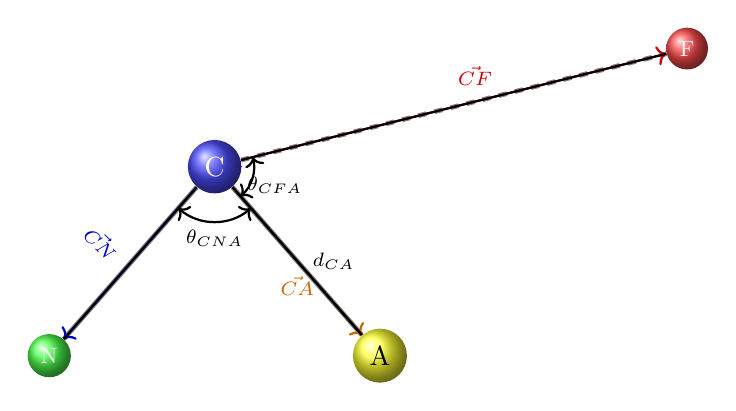
\begin{tikzpicture}[scale=3]
    \node[ball color=blue!70, circle, text=white, scale=1] (C) at (0, 0) {C};
    \node[ball color=green!70, circle, text=white, scale=0.8] (N49) at (-0.7, -0.8) {N};
    \node[ball color=red!70, circle, text=white, scale=0.8] (F) at (2, 0.5) {F};
    \node[ball color=yellow!80, circle, text=black, scale=1] (A) at (0.7, -0.8) {A};
    % Draw bonds
    \draw[gray, line width=0.6mm] (C) -- (N49);
    \draw[gray, line width=0.6mm] (C) -- (A);
    \draw[gray, line width=0.6mm, dashed] (C) -- (F);
    % Draw vectors
    \draw[->, thick, blue!80!black] (C) -- (N49) node[pos=0.5, left=3pt, font=\scriptsize, rotate=-45] {$\vec{CN}$};
    \draw[->, thick, red!80!black] (C) -- (F) node[pos=0.55, above=2pt, font=\scriptsize] {$\vec{CF}$};
    \draw[->, thick, orange!80!black] (C) -- (A) node[pos=0.5, below=2pt, font=\scriptsize] {$\vec{CA}$};
    \draw[black, dashed] (C) -- (A) node[midway, below=2pt, right=2pt, font=\scriptsize] {$d_{CA}$};
    % Draw angles using TikZ angles library
    \draw [thick] 
      (N49) -- (C) -- (A)
      pic["$\theta_{CNA}$", draw=black, angle eccentricity=1.3, angle radius=7mm, font=\scriptsize, <->, fill=none] {angle=N49--C--A};
    \draw [thick]
      (A) -- (C) -- (F)
      pic["$\theta_{CFA}$", draw=black, angle eccentricity=1.6, angle radius=5mm, font=\scriptsize, <->, fill=none] {angle=A--C--F};
  \end{tikzpicture}
  \begin{itemize}
    \item \textbf{Features}: \( \|\vec{CA}\| \), \( \theta_{CAF} \), \( \theta_{CAN} \) (signed angles).
    \item \textbf{Invariance}: This ensures Translation and rotation invariant.
  \end{itemize}
\end{frame}

\begin{frame}{Transformer Architecture}
  \begin{center}
    \begin{adjustbox}{max width=\textwidth}
      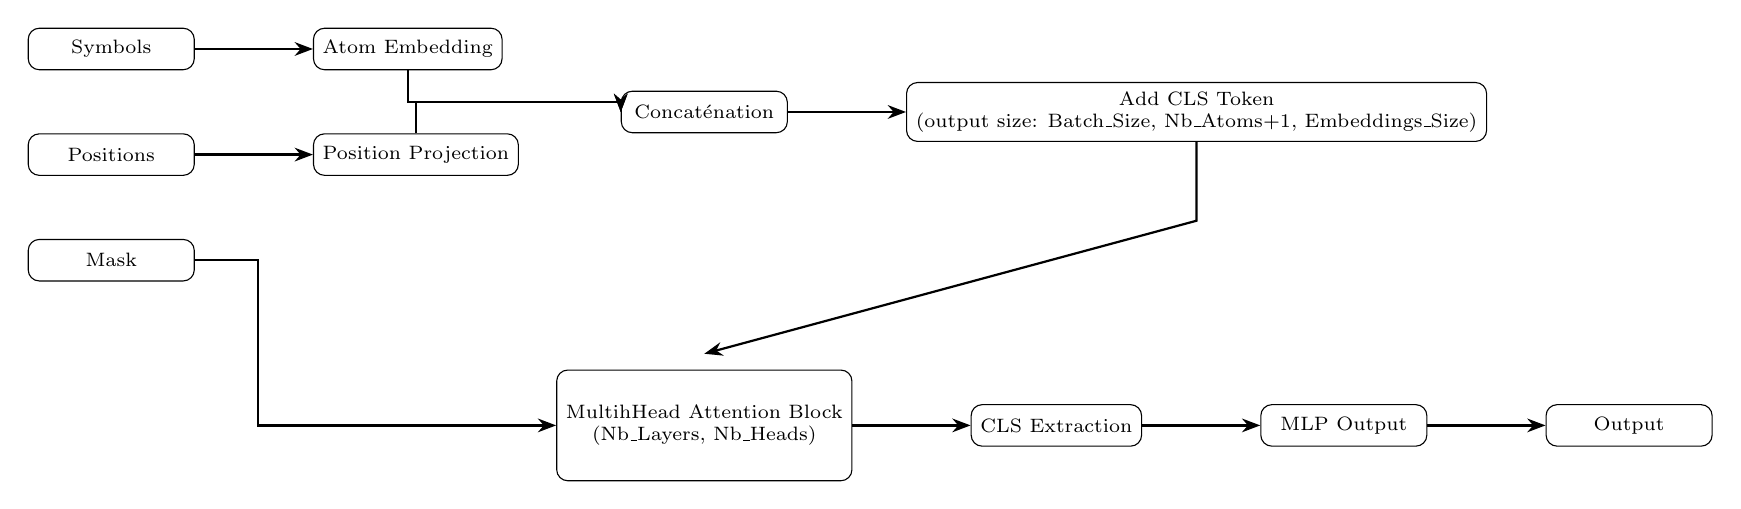
\begin{tikzpicture}[box/.style={rectangle, draw, rounded corners, minimum height=1.5em, minimum width=6em, align=center, font=\scriptsize}, arrow/.style={-Stealth, thick}, node distance=0.8cm and 1.5cm]
        \node[box] (symbols) {Symbols};
        \node[box, below=of symbols] (positions) {Positions};
        \node[box, below=of positions] (mask) {Mask};
        \node[box, right=of symbols] (atom_emb) {Atom Embedding};
        \node[box, right=of positions] (pos_emb) {Position Projection};
        \node[box, right=of atom_emb, yshift=-0.8cm] (concat) {Concaténation};
        \node[box, right=of concat] (cls) {Add CLS Token\\{\scriptsize (output size: Batch\_Size, Nb\_Atoms+1, Embeddings\_Size)}};
        \node[box, below=3cm of concat, minimum height=4em] (attn) {MultihHead Attention Block\\(Nb\_Layers, Nb\_Heads)};
        \node[box, right=of attn] (cls_extract) {CLS Extraction};
        \node[box, right=of cls_extract] (mlp) {MLP Output};
        \node[box, right=of mlp] (output) {Output};
        \draw[arrow] (symbols) -- (atom_emb);
        \draw[arrow] (positions) -- (pos_emb);
        \draw[arrow] (atom_emb.south) -- ++(0,-0.4) -| (concat.west);
        \draw[arrow] (pos_emb.north) -- ++(0,0.4) -| (concat.west);
        \draw[arrow] (concat) -- (cls);
        \draw[arrow] (mask.east) -- ++(0.8,0) |- (attn.west);
        \draw[arrow] (cls.south) -- ++(0,-1) -- ([yshift=2mm]attn.north);
        \draw[arrow] (attn) -- (cls_extract);
        \draw[arrow] (cls_extract) -- (mlp);
        \draw[arrow] (mlp) -- (output);
      \end{tikzpicture}
    \end{adjustbox}
  \end{center}
  \begin{itemize}
    \item \textbf{Components}: Atom embedding, position projection, CLS token, multi-head attention, MLP output.
    \item \textbf{Hyperparameters}: Embedding size = 1024, 30 heads, 1 attention block.
    \item \textbf{Number Of Parameters}: $163 000 000$ parameters.
  \end{itemize}



\end{frame}


% \begin{frame}{Invariance of the model}
%   \begin{itemize}
%     \item \textcolor{red}{\textbf{Translation Invariance}}: Model predictions remain unchanged under spatial translations of the input.

%     \vspace{0.2cm}

%     \item \textcolor{red}{\textbf{Rotation Invariance}}: Model predictions are invariant to rotations of the input configuration.

%     \vspace{0.2cm}

%     \item \textcolor{red}{\textbf{Permutation Invariance}}: Model treats input atoms as indistinguishable, ensuring consistent predictions regardless of atom ordering.
%   \end{itemize}
% \end{frame}

\begin{frame}{Permutation Invariance}
  \begin{itemize}
    \item \textcolor{red}{\textbf{Definition}}: Model predictions are unchanged when the order of input atoms is permuted.
    \vspace{0.3cm}
    \item \textcolor{red}{\textbf{Implementation}}: 
      \begin{itemize}
        \item Atoms treated as independent tokens, no positional encoding.
        \vspace{0.3cm}
        \item Atoms sorted by distance from the center atom to ensure consistent input structure.
      \end{itemize}
    \vspace{0.3cm}
    \item \textcolor{red}{\textbf{Impact}}: Predictions depend only on relative geometric information, not on arbitrary atom ordering.
  \end{itemize}
\end{frame}

\begin{frame}{Translation Invariance}
  \begin{itemize}
    \item \textcolor{red}{\textbf{Definition}}: Model predictions remain consistent under spatial translations of the molecule.
    \vspace{0.3cm}
    \item \textcolor{red}{\textbf{Mathematical Proof}}:
    \vspace{0.3cm}
      \begin{itemize}
        \item Distance \( \|\vec{CA}\| = \sqrt{(x_A - x_C)^2 + (y_A - y_C)^2 + (z_A - z_C)^2} \) is invariant as translation terms cancel.
        \vspace{0.3cm}
        \item Angles \( \theta_{CAF} \), \( \theta_{CAN} \) depend on vectors unchanged by translation (\( \vec{CA}' = \vec{CA} \)).
        \vspace{0.3cm}
        \item Nearest and furthest atoms remain the same as distances \( \|\vec{Ci}\| \) are preserved.
      \end{itemize}
    \vspace{0.3cm}
    \item \textcolor{red}{\textbf{Impact}}: Model is invariant to translations, ensuring consistent predictions regardless of molecular position in space.
  \end{itemize}
\end{frame}

\begin{frame}{Rotation Invariance}
  \begin{itemize}
    \item \textcolor{red}{\textbf{Definition}}: Model predictions are invariant to rotations of the molecule around any axis.
    \vspace{0.3cm}
    \item \textcolor{red}{\textbf{Mathematical Proof}}:
      \begin{itemize}
        \item Norm invariance: \( \|\vec{CA}'\| = \|R \vec{CA}\| = \|\vec{CA}\| \), since \( R \) is an orthogonal matrix (\( R^T R = I \)).
        \vspace{0.3cm}
        \item Dot product invariance: For rotated vectors \( \vec{CA}' = R \vec{CA} \), \( \vec{CF}' = R \vec{CF} \),
          \[
          \vec{CA}' \cdot \vec{CF}' = (R \vec{CA})^T (R \vec{CF}) = \vec{CA}^T R^T R \vec{CF} = \vec{CA}^T \vec{CF} = \vec{CA} \cdot \vec{CF}
          \]
        \vspace{0.3cm}
        \item Angles \( \theta_{CAF} \), \( \theta_{CAN} \) preserved since \( \cos(\theta_{CAF}') = \cos(\theta_{CAF}) \).
        \vspace{0.3cm}
        \item Nearest and furthest atoms remain consistent as norms \( \|\vec{CA}\| \) and \( \|\vec{Ci}\| \) are invariant.
      \end{itemize}
    \vspace{0.3cm}
    \item \textcolor{red}{\textbf{Impact}}: Model ensures consistent predictions regardless of molecular orientation.
  \end{itemize}
\end{frame}


\begin{frame}{Training and Results}
  \begin{itemize}
    \item \textcolor{red}{\textbf{Training}}: Adam optimizer, learning rate \( 3 \times 10^{-5} \), 450 epochs.
    \item \textcolor{red}{\textbf{Results}}: Kaggle score = 0.306, indicating good generalization.
    \item \textcolor{red}{\textbf{Loss Evolution}}:
      \begin{center}
        \includegraphics[width=0.6\linewidth]{Images_Ayoub/Training/Transformers/V2/Losses/First_450_Epochs/Loss.png}
        \captionof{figure}{Loss evolution (log scale) for V2 model.}
      \end{center}
    
  \end{itemize}
\end{frame}

\section{Conclusion}
\begin{frame}{Conclusion}
  \vspace{0.2cm}
  \begin{itemize}
    \item \textcolor{red}{\textbf{Summary}}:
      \begin{itemize}
        \item 3D Wavelet Scattering: High-quality invariant features, Kaggle score 0.125.
        \vspace{0.15cm}
        \item Transformer: Invariant geometric features, Kaggle score 0.311.
      \end{itemize}
    \vspace{0.2cm}
    \item \textcolor{red}{\textbf{Key Insights}}: Both approaches ensure invariance, with Transformers excelling in modeling complex interactions.
    \vspace{0.2cm}
    \item \textcolor{red}{\textbf{Future Work}}: Combine GNN and Transformers, explore advanced architectures (Path Advanced Graph Neural Networks).
    \item \textcolor{red}{\textbf{Reference}}: \href{https://arxiv.org/pdf/1905.12712}{arXiv:1905.12712}
      
  \end{itemize}
  \vspace{0.2cm}
\end{frame}

\end{document}